\begin{pa} \label{PA:10.6} 
  Let's consider the function 
  $$
  f(x,y) = x^2 + \frac 12 y^2.
  $$
  A contour plot of $f$ is shown in Figure \ref{F:10.6.preview.1}

  \begin{figure}[ht]
    \begin{center}
      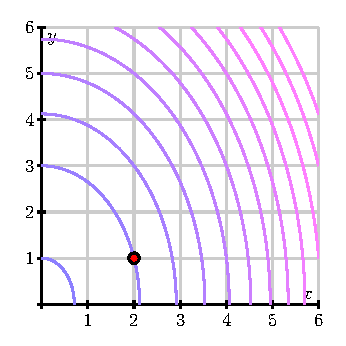
\includegraphics{figures/fig_10_6_preview_1.eps}
    \end{center}
    \caption{A contour plot of $f(x,y)$.}
    \label{F:10.6.preview.1}
  \end{figure}
  \ba
\item Suppose we are moving across the plane and pass through the
  point $(2,1)$ with velocity $\vv=\langle -1,2\rangle$.  Use the Chain
  Rule to determine the rate of change $df/dt$.
\item Let's look at the preceeding computation and rewrite it in a way
  that has geometric meaning:
  \begin{align*}
    \frac{df}{dt} &= \frac{\partial f}{\partial x}(2,1)\frac{dx}{dt} + 
    \frac{\partial f}{\partial y}(2,1)\frac{dy}{dt} \\
    & = \left\langle \frac{\partial f}{\partial x}(2,1),
    \frac{\partial f}{\partial y}(2,1) \right\rangle \cdot
  \left\langle \frac{dx}{dt}, \frac{dy}{dt}\right\rangle \\
    & = \left\langle \frac{\partial f}{\partial x}(2,1),
    \frac{\partial f}{\partial y}(2,1) \right\rangle \cdot \vv.\\
  \end{align*}
  This shows that the rate of change of $f$ is the dot product of a
  vector $ \left\langle \frac{\partial f}{\partial x}, \frac{\partial
    f}{\partial y} \right\rangle$ with the velocity vector.  We call this
  vector the {\em gradient} of $f$ and denote it
  $$
  \nabla f(x,y) = \left\langle \frac{\partial f}{\partial x}(x,y),
  \frac{\partial f}{\partial y}(x,y) \right\rangle.
  $$
  Find the gradient $\nabla f(2,1)$ and sketch this vector on Figure
  \ref{F:10.6.preview.1} with its tail at the point $(2,1)$.

  \item What do you notice about the relationship between the gradient
    vector $\nabla f(2,1)$ and the contour line passing
    through $(2,1)$.

  \item Suppose you are passing through the point $(2,1)$ moving with
    velocity $\vv =\langle -1,4\rangle$.  Sketch this velocity vector
    on Figure \ref{F:10.6.preview.1}.  Then find the rate of change of
    $f$ using the expression
    $$
    \frac{df}{dt} = \nabla f(2,1)\cdot\vv.
    $$
  \item How does the velocity vector $\vv=\langle -1,4\rangle$ that
    you considered in the last part relate to the contour line through
    $(2,1)$.  How does this explain the rate of change $df/dt$ that
    you found?

  \item From Section \ref{S:9.3.Dot_Product}, remember the geometric
    information  conveyed by the dot product.  If $\theta$ is the
    angle between $\nabla f(2,1)$ and the velocity vector $\vv$, then
    $$
    \frac{df}{dt} = \nabla f(2,1)\cdot\vv =
    |\nabla(2,1)||\vv|\cos\theta.
    $$
    Suppose that we move with unit speed;  that is, suppose that
    $|\vv| = 1$.  What value of $\theta$ gives the largest possible
    rate of change $df/dt$?  In what direction should we move if we
    want $f$ to increase as rapidly as possible?
  \item What value of $\theta$ gives the smallest possible rate of
    change $df/dt$?  In what direction should we move if we want $f$
    to decrease as rapidly as possible?
 \ea

\end{pa} \afterpa 